\chapter{The Standard Model and Supersymmetry}
\label{ch:theory} 
\epigraph{\emph{A theory is something nobody believes, except the person who made it. An experiment is something everybody believes, except the person who made it.}} {Albert Einstein}

	\begin{wrapfigure}{R}{.5\textwidth}
		\centering
			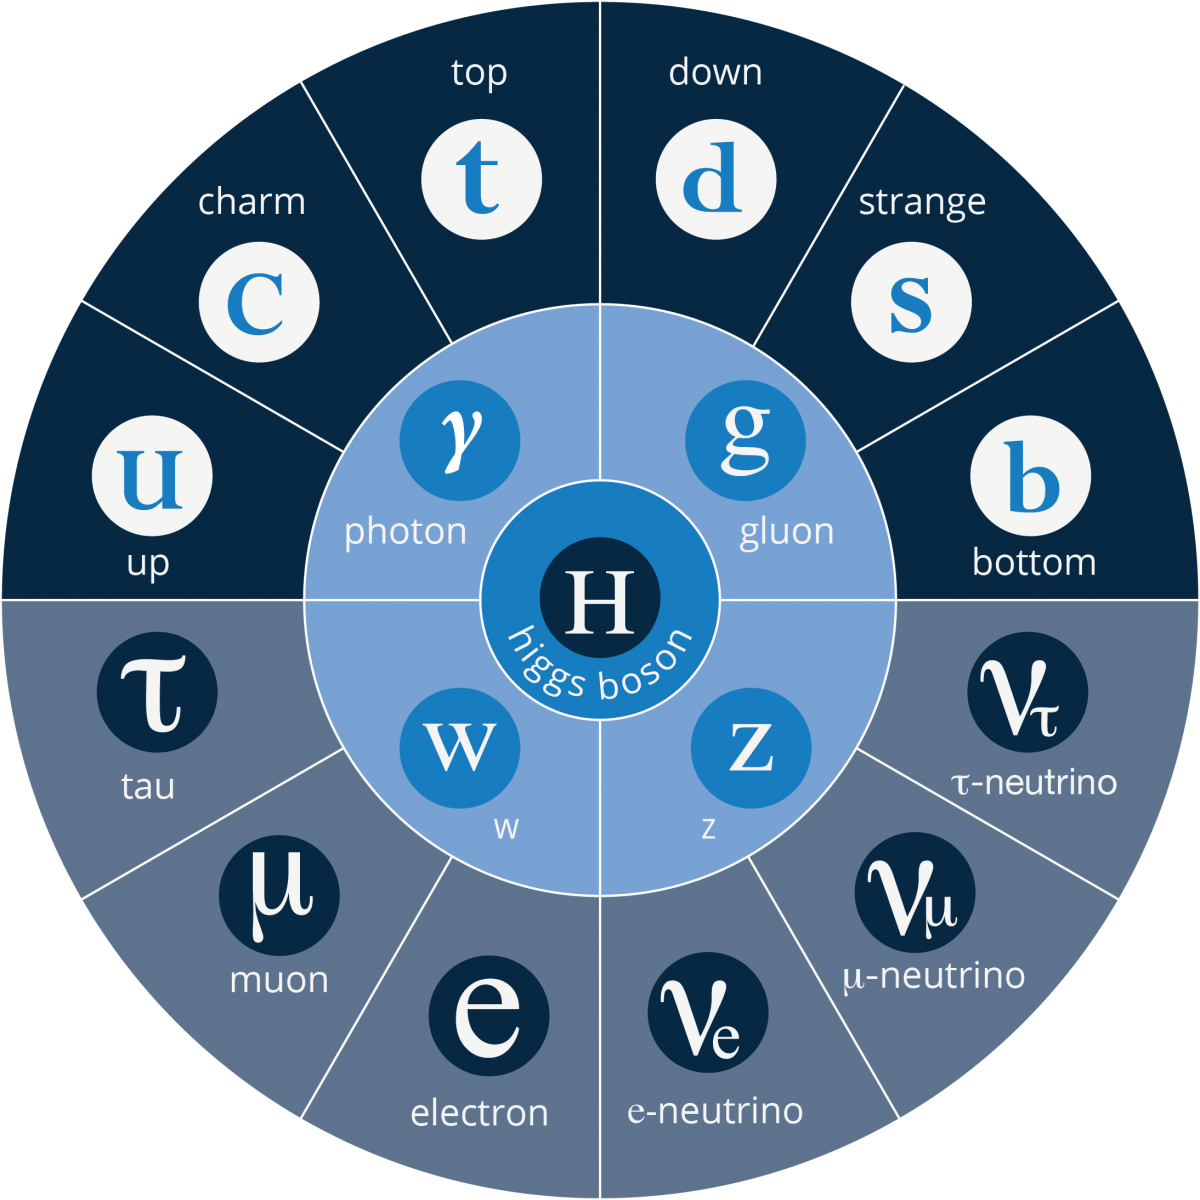
\includegraphics[width=.35\textwidth]{theory/sm}
		\caption{\label{fig:sm_el_part} The elementary particles of the \ac{SM}. From the outermost to the innermost; fermions (quarks, top-half wheel, leptons, bottom-half wheel), vector bosons, and the Higgs boson.}
	\end{wrapfigure}				

	Section~\ref{sec:SMov} presents an overview of the~\ac{SM} of particle physics, together with its limitations (Section~\ref{sec:SMlim}) and the need of an extension. One of the most popular of these extensions, \ac{SUSY}, will be discussed in Section~\ref{sec:SUSY} where an overview of the theory and the motivations behind its success will be presented. The description of the \ac{MSSM} in Section~\ref{sec:MSSM}, and finally the phenomenology of supersymmetry, with particular attention to third-generation supersymmetry - as the most relevant theoretical support to this work - will be discussed in Section~\ref{sec:SUSYPheno}.


	\section{The Standard Model}
	\label{sec:SMov}

		The \ac{SM} is an effective theory that aims to provide a general description of fundamental particles and their interactions. %Unfortunately, our understanding of nature is still limited due to some opened question the SM is not able to answer to.

		The $20^{th}$ century can be considered a quantum revolution. Several experiments led to discoveries which were found to be, together with the formalised theory, a solid base of the \ac{SM} of particle physics and our description of nature. Several particles were first predicted and then experimentally observed \eg\ the \Wboson\ and the \Zboson\ bosons, the $\tau$ lepton,~\cite{Herrero1998}, and more recently the Higgs boson at the \ac{LHC} discovered by the \acs{ATLAS}~\cite{ATLASHiggs2012} and \acs{CMS}~\cite{CMSHiggs2012} collaborations.

		The \ac{SM} is a \ac{QFT} where particles are treated like excitations of quantum fields in a four-dimensional Minkowski space-time~\cite{Peskin1995}. It can describe three of the four fundamental forces; weak, electromagnetic, and strong, but not gravity.

		The most general classification of the elementary particles within the \ac{SM} can be made by means of spin and their behaviour under Poincaré transformations~\cite{Cottingham1998}: \textit{fermions} (leptons and quarks), usually referred to as matter particles, which have half-integer spin values, in unit of $\hslash$, and \textit{bosons}, usually referred to as information carriers, which have integer-spin values. A noteworthy subset of bosons is formed by the Spin-1 bosons, also known as gauge bosons. These can be considered mediators of the forces. Figure~\ref{fig:sm_el_part} displays the elementary particles of the Standard Model known as of today.



		\subsection*{Symmetries and Gauge Groups}

			In 1915, the German mathematician and theoretical physicist Emmy Noether (23 March 1882 – 14 April 1935) proved that every differentiable symmetry of the action of a physical system - defined as the integral over space of a Lagrangian density function $S = \int \mathcal{L}\, dt$ - has a corresponding conservation law~\cite{lederman2004symmetry}. More generally, a symmetry is a property of a physical system and under certain transformations this property is preserved. 

			A gauge theory in \ac{QFT}, is a theory in which the Lagrangian is invariant under a continuous group of local transformations. Group theory was adopted to describe the symmetries conserved in the \ac{SM}. The gauge group of the \ac{SM} is the \emph{Lie Group} which contains all the transformations between possible gauges~\cite{Cottingham1998}. The Lie algebra of group generators is associated to any Lie group and for each group generator there emerges a corresponding field, called the gauge field, and the quanta of such fields are called \emph{gauge bosons}.
			
			The three \ac{SM} interactions can therefore be mathematically described by the following:

			\begin{equation}
			\label{eq:SM_gaugeSym}
				U(1)_Y \otimes SU(2)_L \otimes SU(3)_C
			\end{equation}

			\noindent Here, $Y$ is the weak hypercharge, used to estimate the correlation between the electric charge ($Q$) and the third component of the weak isospin ($I_3$) via the relation $Q = I_3 + Y/2$. $I_3$ can either be $\pm 1/2$ or $0$ for left-handed and right-handed particles, respectively, $L$ the left-handedness, and $C$ the colour charge. 

			\ac{QED} is an Abelian gauge theory described by the symmetry group $U(1)$. The electromagnetic four-potential is its gauge field and the photon its gauge boson~\cite{Pich2012}. The interactions between charged fermions occurs by the exchange of a massless photon. 

			The weak interaction is described by the non-Abelian gauge group $SU(2)$. The $SU(2)$ generators are the massless gauge bosons $W_{\mu}^{\alpha = 1,\dots,3}$ and they violate parity by acting only on left-handed particles. As a consequence of non-Abelianity, $SU(2)$ gauge bosons can self-interact as the generator commutators are non-vanishing. Additionally, quarks can also interact through weak interaction as mixtures of \ac{SM} eigenstates as described by the CKM matrix~\cite{PDG}.

			Finally, the strong interaction, described by the symmetry group $SU(3)$, has eight massless gauge bosons, the gluons, $G_{\mu}^{\alpha=1,\dots,8}$, which can be exchanged between quarks and can also self-interact. 



		\subsection*{Fermions}

			There are twelve fermions in the \ac{SM}: six quarks and six leptons. In particular, fermions can be grouped into three generations. Each generation contains four particles; one up- and one down-type quark, one charged lepton and one neutral lepton. The masses of the charged leptons and quarks increase with the generation. The six quarks of the \ac{SM} can be grouped into three $SU(2)$ doublets;

			\begin{equation*}
			\label{eq:quark_doublets}
				\begin{pmatrix} u \\ d \end{pmatrix}, \qquad 
				\begin{pmatrix} c \\ s \end{pmatrix}, \qquad 
				\begin{pmatrix} t \\ b \end{pmatrix}
			\end{equation*}

			\noindent The up-type quarks (\textit{up, charm, top}) have charge $+\frac{2}{3}e$ and the down-type quarks (\textit{down, strange, beauty/bottom}) have charge $-\frac{1}{3}e$, where $e$ is the electron charge. Quarks also have another quantum number, the colour charge, that can be seen as the analogue of the electric charge. The colour charge exists in three different states (\textit{red}, \textit{green} and \textit{blue}), but quarks cannot propagate as free particles. They rather group to form hadronic matter, also known as \emph{hadrons}. There are two kinds of hadrons; mesons and baryons. Mesons are quark-antiquark systems, \eg\ the pion, and baryons are three-quark system, \eg protons and neutrons. Quarks and anti-quarks have a baryon number of $\frac{1}{3}$ and $-\frac{1}{3}$, respectively.

			There are six leptons and they can be classified in charged leptons (electron $e$, muon $\mu$, tau $\tau$) and neutral leptons (electron neutrino $\nu_e$, muon neutrino $\nu_{\mu}$, tau neutrino $\nu_{\tau}$):
			
			\begin{equation*}
			\label{eq:lepton_flavor_doublets}
				\begin{pmatrix} \nu_e      \\ e^-    \end{pmatrix}, \qquad
				\begin{pmatrix} \nu_{\mu}  \\ \mu^-  \end{pmatrix}, \qquad
				\begin{pmatrix} \nu_{\tau} \\ \tau^- \end{pmatrix}
			\end{equation*}

			\noindent Each lepton has a characteristic quantum number, called lepton number ($L$). Negatively (positively) charged leptons have $L=-1$ ($L=1$) and neutral leptons have $L=1$. The lepton number is conserved in all the interactions. 



		\subsection*{Forces of Nature}

			Forces in the \ac{SM} are described by gauge theories, where the interactions are mediated by a vector gauge boson. 

			\ac{QED} describes the electromagnetic force, which only affects quarks and charged leptons (neutrinos are instead affected by the weak force, mediated by the $\Wboson^{\pm}$ and $\Zboson^0$ bosons), and it is mediated by the photon ($\gamma$).

			The weak interaction is associated with \textit{handedness} \ie, the projection of a particle spin onto its direction of motion. Both leptons and quarks have left- and right-handed components. However, only the left-handed (right-handed) component for neutrinos (anti-neutrinos) has been observed. This means that nature prefers to produce left-handed neutrinos and right-handed anti-neutrinos, which is the so-called \textit{parity violation}~\cite{Weinberg:1996kr}. 

			The strong interaction, mediated by the gluon (electrically neutral and massless), is described by \ac{QCD}. Its coupling ($\alpha_s)$ increases with increasing distance and is smaller at short range. In particular, $\alpha_s$ evolves as a function of the transferred four-momentum squared, $Q^2$, as follows: 

			\begin{equation}
				\label{eq:alpha_s}
				\alpha_s (Q^2) \propto \displaystyle \frac{1}{n_f \log (\frac{Q^2}{\Lambda_{\mathrm{QCD}}^2})} 
			\end{equation}

			\noindent where $n_f$ is the number of quarks with mass below $Q^2$ and $\Lambda_{\mathrm{QCD}}$ is the \ac{QCD} characteristic scale. Equation~\ref{eq:alpha_s} shows that $\alpha_s$ decreases as a function of $\Lambda_{\mathrm{QCD}}$, but at the same time it quickly diverges when $Q^2$ gets closer to $\Lambda$. In other words, as the condition $\alpha_s \muchless 1$ only holds for $Q^2 \gg \Lambda_{\mathrm{QCD}}$, \ac{QCD} can be treated perturbatively\footnote{Perturbation theory (quantum mechanics) is an approximation to describe a complicated quantum system in terms of a simpler one.} only at high energy scales\footnote{Perturbation theory can only be used when the coupling constant (expansion parameter) is small.}. Furthermore, \ac{QCD} has three important features:

			\begin{itemize}
				\item \emph{confinement}: quarks or gluons cannot be observed as free particles, but only colourless “singlet” states can be observed as “jets”, namely collimated cone-shaped sprays of hadrons; 

				\item \emph{asymptotic freedom}: interactions between quarks and gluons become weaker as the energy scale increases and the corresponding length scale decreases, as $\alpha_s \to 0$ for $Q^2 \to \infty$~%\cite{PhysRevLett.30.1343};

				\item \emph{hadronisation}: when quarks or gluons are pulled apart, the production of pairs of hadrons, produced from the vacuum, is energetically preferred to an increase in distance.
			\end{itemize}

			Table~\ref{tab:interactions} summarises the forces described in the \ac{SM} and the main characteristics of the mediators. The gravitational force is believed to be mediated by the graviton but, as already mentioned, since it is not included in the \ac{SM} it will not be further discussed.

			\begin{table}[!htb]\centering\caption{Forces and mediators described by the \ac{SM}}							
				\begin{tabular}{ccccc}
					\toprule
					\textbf{Force} & \textbf{Name} & \textbf{Symbol} & \textbf{Mass} [\GeV]& \textbf{Charge} \\ 
					\toprule
					Electromagnetic & Photon & $\gamma$ & 0 & 0 \\ \midrule
					\multirow{2}{*}{Weak} & W & $\Wboson^{\pm}$ & $80.398$ & $\pm e$ \\
					& Z & $\Zboson^0$ & $91.188$ & 0 \\\midrule
					Strong & Gluon & $g$ & $0$ & $0$ \\\bottomrule
				\end{tabular}						
			\label{tab:interactions} 
			\end{table}


		\subsection{Electroweak Symmetry Breaking and the Higgs mechanism}
		\label{sec:ewksb}

			In 1979 Sheldon Glashow, Abdus Salam, and Steven Weinberg were awarded the Nobel Prize in Physics for their contributions to the so-called electroweak unification~\cite{Glashow:1961tr,SALAM1964168,PhysRevLett.19.1264}. In the mathematical description of the \ac{SM} in~\ref{eq:SM_gaugeSym}, the electroweak interaction is described by $U(1)_Y \otimes SU(2)_L$. 

			The four electroweak physical bosons $\Wboson^{\pm}$, \Zboson\ and $\gamma$ are related to the four unphysical gauge bosons $W_{\mu}^{\alpha = 1,2,3}$ and $B_\mu$. In particular, to obtain the physical bosons the gauge bosons have to mix as follows;

			\begin{equation}
			\label{eq:photon}
				A_{\mu} = W_{\mu}^3 \sin\theta_W  + B_{\mu}\cos \theta_W 
			\end{equation}
			\begin{equation}
			\label{eq:Zboson}
				Z_{\mu} = W_{\mu}^3\cos\theta_W  - B_{\mu} \sin \theta_W
			\end{equation}
			\begin{equation}
			\label{eq:Wboson}
				W_{\mu}^\pm = \frac{1}{\sqrt{2}} \displaystyle \left ( W_{\mu}^1 \mp i W_{\mu}^2 \right )
			\end{equation}

			\noindent Here, $\theta_W$ is the so-called \emph{Weinberg angle} which is the angle by which spontaneous symmetry breaking rotates the original gauge bosons $\Wboson_{\mu}^3$ and $B_{\mu}$ into the physical \Zboson\ and $\gamma$. $A_\mu$ and $Z_\mu$ are the photon and the \Zboson\ boson fields, respectively. The $\theta_W$ angle can be experimentally determined in terms of the coupling strengths, of the $B_{\mu}(g_1)$ and the $W_{\mu}^\alpha (g_2)$ to the fermions, using the relation $\tan\theta_W = g_1 / g_2 $. 

			The mass terms for both gauge bosons and fermionic fields are forbidden by the electroweak gauge as they are not invariant under gauge transformations. Nonetheless, it was experimentally proven that \Wboson\ and \Zboson\ bosons have mass~\cite{Pich2012}, therefore in order for the \ac{SM} assumption to hold, the electroweak symmetry must be broken. 

			The \ac{SM} Lagrangian can be written as the sum of the various Lagrangians describing the three interactions and the masses of the elementary particles as follows:

			\begin{equation}
			\label{eq:SM_Lagrangian}
				\mathcal{L_{\mathrm{SM}}} = \mathcal{L_{\mathrm{EWK}}} + \mathcal{L_{\mathrm{QCD}}} + \mathcal{L_{\mathrm{Mass}}}
			\end{equation}

			\noindent In order for the \ac{SM} Lagrangian to remain a re-normalisable theory, the mass terms $\left ( \mathcal{L_{\mathrm{Mass}}} \right )$ cannot be inserted by hand. A mechanism, that can preserve the gauge symmetry in the \ac{SM} and can solve the inconsistency arisen from the mass difference between the gauge bosons and the physical ones is needed. A British theoretical physicist, Peter Higgs (29 May 1929, Newcastle upon Tyne, UK), came up with a brilliant solution for which he was awarded the Nobel Prize in Physics in 2013. Higgs proposed~\cite{Higgs1964} that broken symmetry in the electroweak theory could explain the origin of masses of elementary particles, and in particular of \Wboson\ and \Zboson\ bosons. The mechanism introduces a scalar field, known as the Higgs field, thought to couple to both massive fermions and bosons. The $SU(2)$ doublet is then introduced in the \ac{SM};

			\begin{equation}
			\label{eq:Higgs_field}
				\phi = 
				\begin{pmatrix}
					\phi^+ \\ \phi^0
				\end{pmatrix} 
			\end{equation}

			\noindent with $\phi^+$ and $\phi^0$ generic complex fields: 

			\begin{equation}
				\phi^+ = \frac{\phi_1 + i \phi_2}{\sqrt{2}},  \qquad \phi^0 = \frac{\phi_3 + i \phi_4}{\sqrt{2}}
			\end{equation}

			\noindent Consider a Lagrangian of the form: 

			\begin{equation}
			\label{eq:Higgs_lagrangian}
				\mathcal{L_{\mathrm{Higgs}}} = ( \partial_{\mu} \phi )^* \left ( \partial^{\mu} \phi \right ) - V(\phi)
			\end{equation}

			\noindent where $V(\phi)$ is now the Higgs potential. Re-normalisability and $SU(2)_L \otimes U(1)_Y$ invariance require the Higgs potential to be of the following form: 

			\begin{equation}
			\label{eq:Higgs_potential}
				V(\phi) = \mu^2  \phi^\dagger \phi + \lambda \left ( \phi^\dagger \phi \right )^2 
			\end{equation}

			\noindent The Lagrangian in Equation~\ref{eq:Higgs_lagrangian} is the Higgs Lagrangian if $\phi$ is chosen to be the following:

			\begin{equation*}
				\phi = 
				\begin{pmatrix}
					\phi^+ \\ \phi^0
				\end{pmatrix} 
				=
				\begin{pmatrix}
					G^+ \\ \frac{1}{\sqrt{2}} \left ( v + H + iG^0 \right )
				\end{pmatrix}
			\end{equation*}

			\noindent Here, the complex scalar field $G^\pm$ and the real scalar field $G^0$ correspond to Goldstone bosons, and the real scalar field $H$ is the \ac{SM} Higgs boson field~\cite{Goldstone1962}. These massless scalars are absorbed due to the gauge transformations by the electroweak gauge bosons of the \ac{SM}:

			\begin{equation}
			\label{eq:Higgs_doublet}
				\phi = 
				\begin{pmatrix}
					\phi^+ \\ \phi^0
				\end{pmatrix} 
				=
				\begin{pmatrix}
					0 \\ \frac{1}{\sqrt{2}} \left ( v + H \right )
				\end{pmatrix}
			\end{equation}

			\begin{wrapfigure}{R}{.5\textwidth}
				\centering
				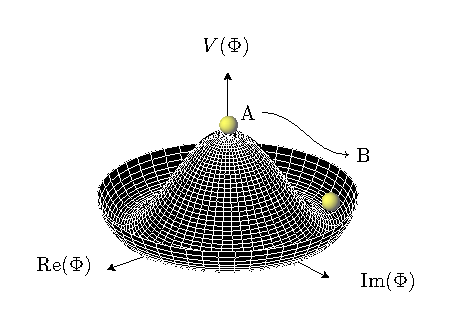
\includegraphics[width=.4\textwidth]{HiggsPotential/HiggsPotential}
				\caption{\label{fig:higgs_potential}The Higgs potential in the complex plane.} %Any given point around the bottom of the hat gives the lowest-energy state.}
			\end{wrapfigure}

			The Higgs potential in Equation~\ref{eq:Higgs_potential} is displayed in Figure~\ref{fig:higgs_potential} if $\lambda$ and $\mu$ are chosen to be real. Such potential has a non-zero ground state, $v$, also known as \ac{VEV}:

			\begin{equation}
			\label{eq:Higgs_vev}
				\phi_0 = 
				\begin{pmatrix}
					0 \\ \frac{1}{\sqrt{2}} v
				\end{pmatrix}
			\end{equation}

			\noindent Such representation remains invariant under $U(1)$ allowing electric charge conservation. However, the \ac{SM} gauge symmetry~\ref{eq:SM_gaugeSym} is broken into $SU(2)_L \otimes U(1)_Y$.

			In summary, to generate particle masses gauge symmetry must be broken. However, in order for the theory to remain re-normalisable, the global Lagrangian symmetry must be preserved. This can be solved introducing the concept of \emph{spontaneous} symmetry breaking (SSB): a mechanism that allows a symmetric Lagrangian, but not a symmetric vacuum. In particular, given a Lagrangian invariant under a certain transformation, $T_X$, and a generic set of states, that transform under $T_X$ as the elements of a multiplet, the symmetry is spontaneously broken if one of those states is arbitrarily chosen as the ground state of the system. 
			%The Higgs-field \ac{VEV} is not invariant under gauge transformations. In fact, it spontaneously breaks the gauge symmetry leaving the symmetry of the model untouched. 
			The interaction of the Higgs field with the $SU(2) \otimes U(1)$ gauge fields, $W_\mu^{\alpha =1,2,3}$, result in the three gauge bosons fields acquiring mass whilst the $A_\mu$ field remains massless. 



		\subsection{Limitations of the Standard Model}
		\label{sec:SMlim}

			The \ac{SM} has been extensively validated at the \ac{LEP} at CERN (Geneva), Tevatron at Fermilab (Chicago, IL), and SPEAR/PEP at SLAC (Stanford, CA). The first Run of the \acs{LHC} (Run 1) extended the validation beyond the energy limits of previous colliders as shown in Figure~\ref{fig:ATLAS_a_SMSummary_TotalXsect}: the agreement, between the measured production cross-section of various \ac{SM} processes and the \ac{SM} predictions, looks very good. However, there are some fundamental questions that still have no answer.

			\begin{figure}[!htb]
				\centering
				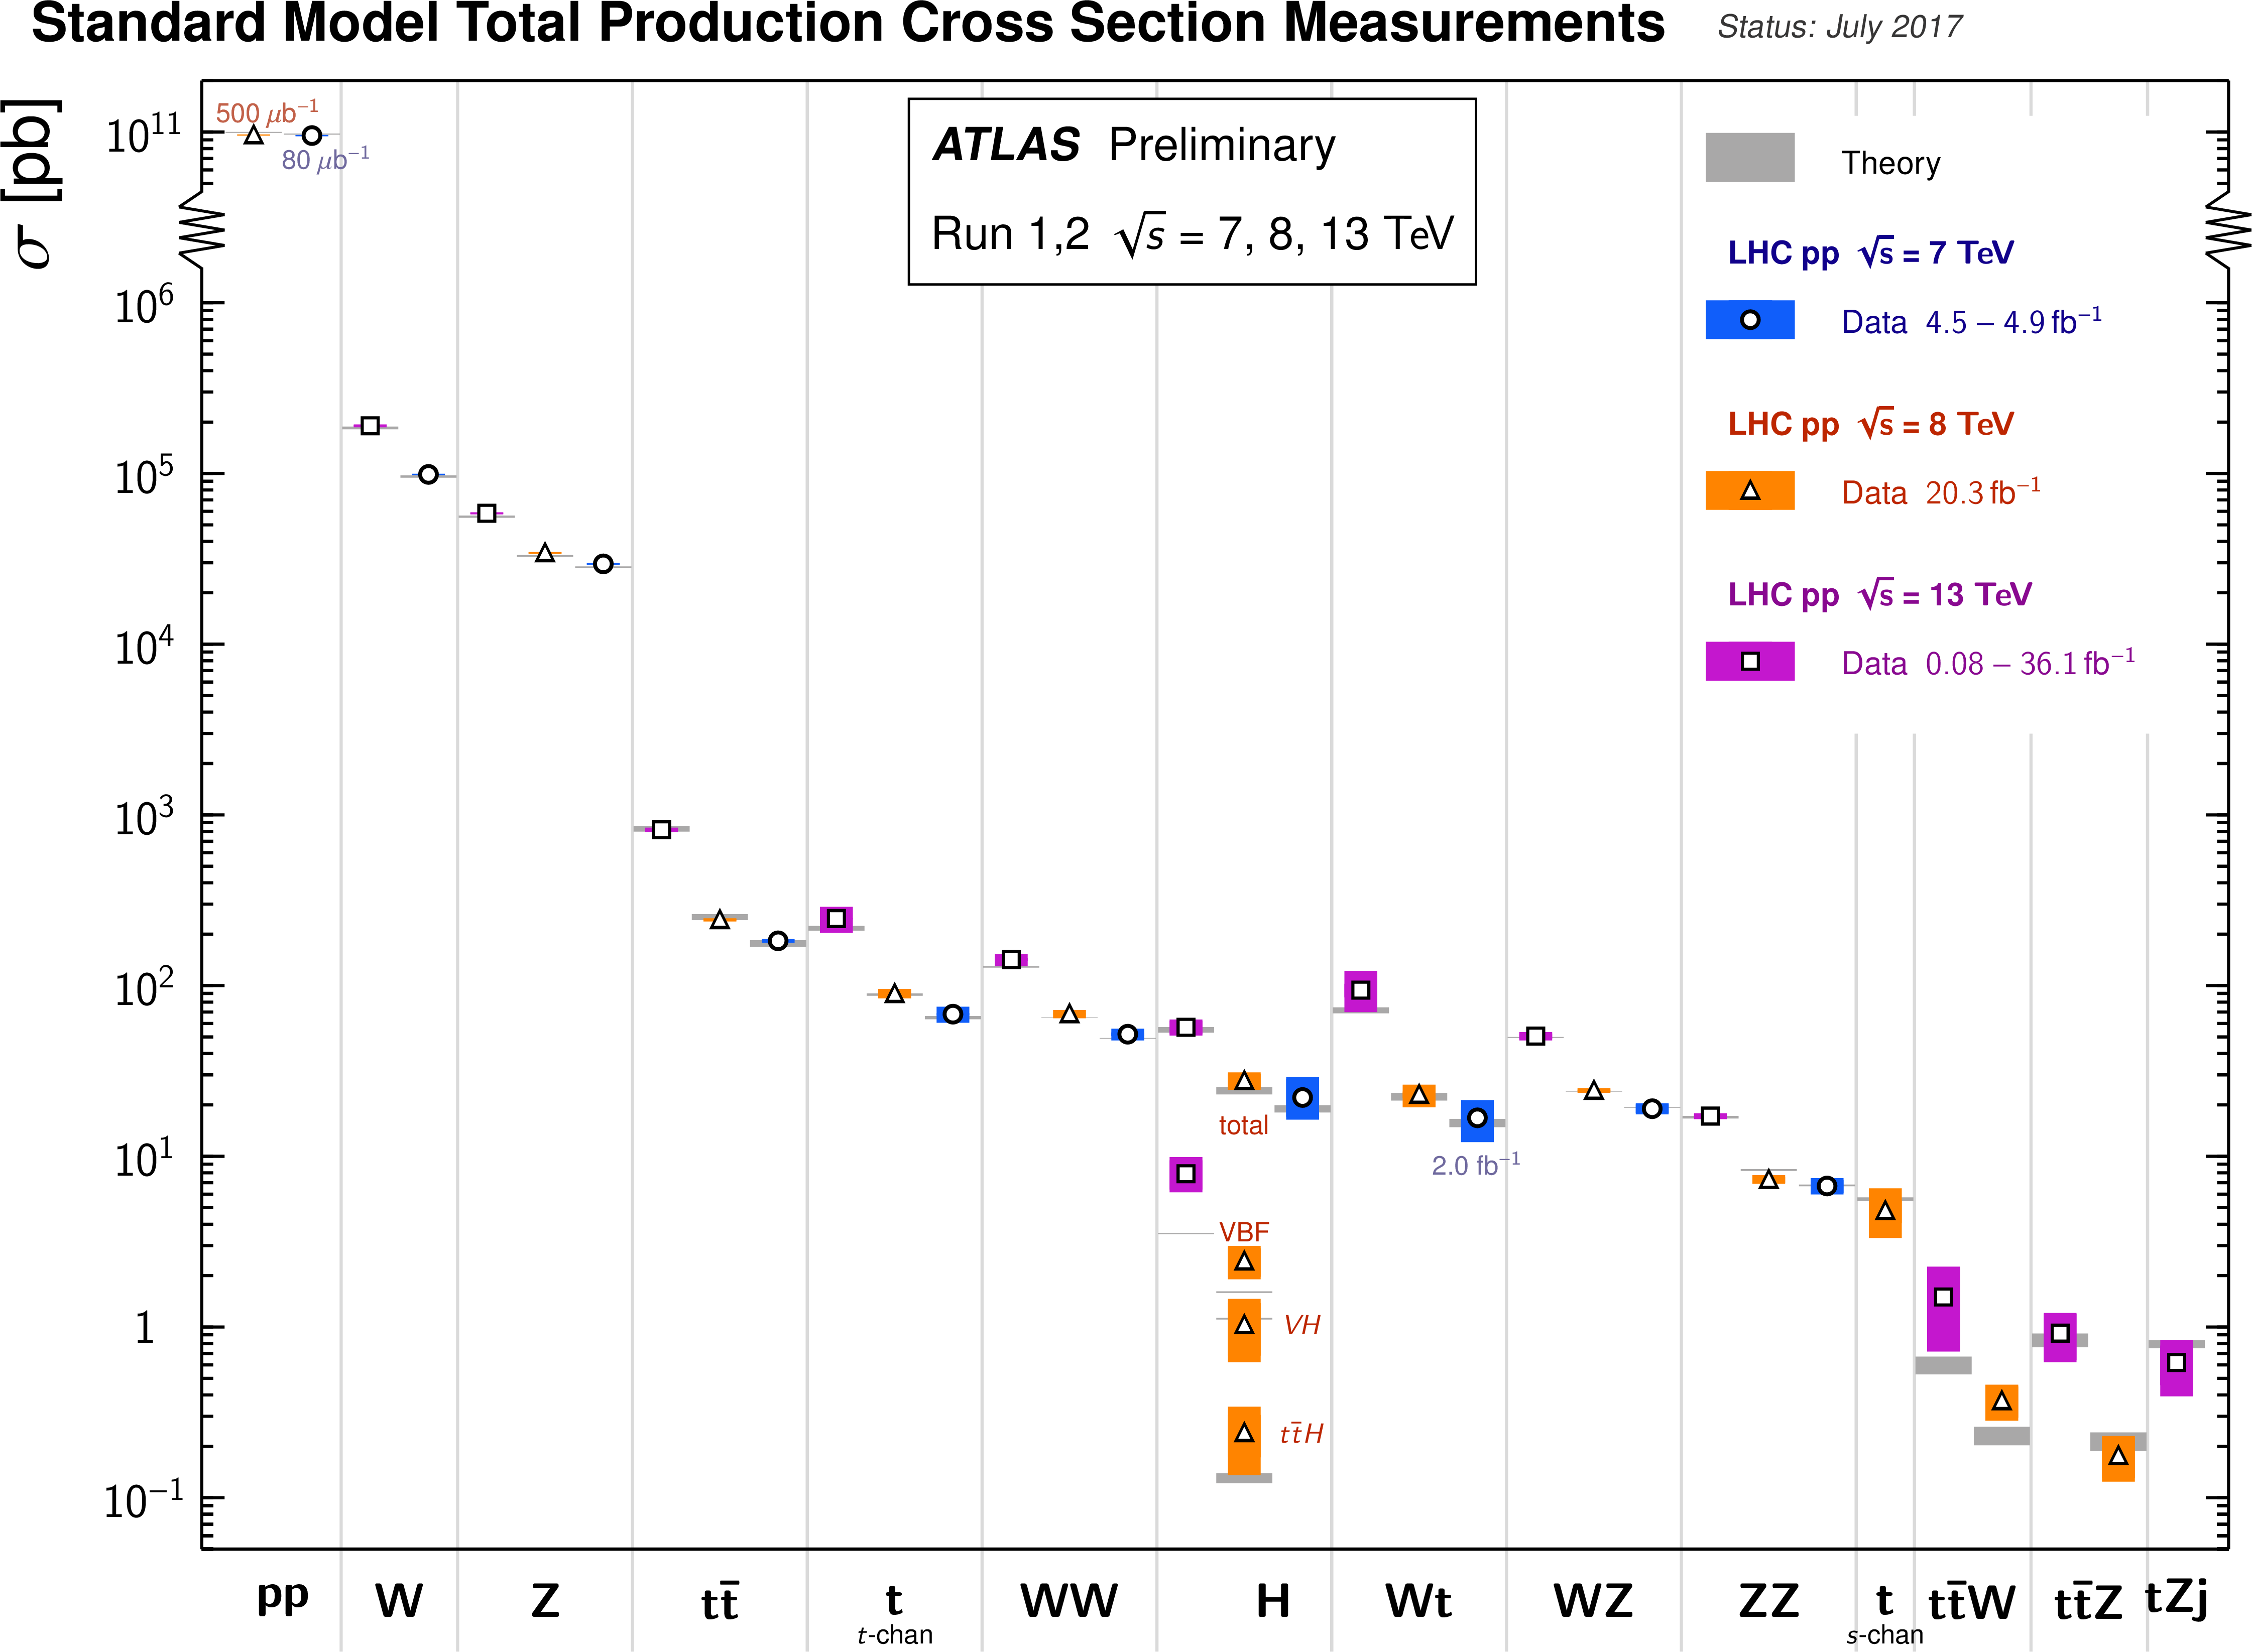
\includegraphics[width=\textwidth]{theory/ATLAS_a_SMSummary_TotalXsect}
				\caption{\label{fig:ATLAS_a_SMSummary_TotalXsect} Summary of several \ac{SM} total production cross-section measurements, corrected for leptonic branching fractions, compared to the corresponding theoretical expectations. All theoretical expectations were calculated at NLO or higher. The luminosity used for each measurement is indicated close to the data point. Uncertainties for the theoretical predictions are quoted from the original ATLAS papers. They were not always evaluated using the same prescriptions for PDFs and scales. Not all measurements are statistically significant yet~\cite{ATLAS_a_SMSummary_TotalXsect}.}
			\end{figure}



		\subsubsection*{Hierarchy Problem}

			Due to the coupling of the Higgs field to the fermionic fields, the one-loop corrections to the Higgs mass receive several contributions~\cite{Weinberg1976}. In particular, looking at Figure~\ref{fig:higgs_f_coupling}: 

			\begin{equation}
				\label{eq:mH_fermionic_contribution}
				\Delta m_H^2 = - \frac{ | \lambda_f  |^2}{8 \pi ^2} \Lambda_{\mathrm{UV}}^2 + \dots 
			\end{equation}
 	
			\noindent where, $\lambda_f$ is the coupling constant to the fermionic field; $\Delta m_H^2$ is the difference between the observed Higgs mass $m_H^2$ and the bare mass, $m_H^0$ (Lagrangian parameter); $\Lambda_{\mathrm{UV}}$ is the ultraviolet momentum cut-off, selected to be at the Planck scale ($\sim 2 \cdot 10^{18} \gev$), at which a \ac{QFT} description of gravity is believed to become possible. The correction to the Higgs mass will be around 30 orders of magnitude larger than Higgs mass itself, in opposition to what has been measured. This difference just mentioned, between the electroweak scale and the Planck scale arisen from the quantum corrections to the Higgs mass, is the so-called Hierarchy Problem~\cite{Weinberg1976}.

			\begin{figure}
				\centering
				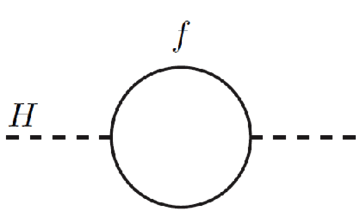
\includegraphics[width=.3\textwidth]{theory/1loopFermionicCorrections}
				\caption{\label{fig:higgs_f_coupling} One-loop quantum corrections to the Higgs mass. A fermion correction with coupling $\lambda_f$.}
			\end{figure}



		\subsubsection*{Neutrino Masses}

			The Super-Kamiokande Collaboration in 1998~\cite{SK1998}, and SNO Collaboration in 2001~\cite{SNO2001}, have provided measurements of the neutrino flux from solar and atmospheric sources. 
			The Nobel Prize in Physics 2015 was awarded jointly to Takaaki Kajita and Arthur B. McDonald ``for the discovery of neutrino oscillations, which shows that neutrinos have mass''~\cite{Nobel2015}. Such feature contradicts the description of the neutrinos in the \ac{SM}, which are assumed to be massless, therefore there needs to be a mechanism that generates neutrino masses. One possibility would be to add Majorana mass terms or adding additional right-handed neutrinos with a very heavy mass, known as the see-saw mechanism~\cite{Akhmedov1999}.


		\subsubsection*{Dark Matter}

			Although \ac{DM} has never been directly observed, its existence is inferred from its gravitational effects. For example, looking at galaxies rotation, it was observed that the rotation speed was higher than expected, given the amount of visible matter~\cite{Rubin1970}. Two different reasoning arose during the last century to justify such effect: there is either matter that cannot be seen by us (in terms of visible light), which contributes to the galactic mass, or the general relativity works differently at galactic distances. The former is believed to be the most likely explanation and it implies the existence of new particles which do not interact via electromagnetic interaction, the so-called \acp{WIMP}~\cite{oro44361}.



	\section{Supersymmetry and the MSSM}
	\label{sec:SUSY}	

		One of the main motivations for \ac{SUSY} is the cancellation of quadratic divergences to $\Delta m_H^2$ via the introduction of the so-called \ac{SUSY} particles, with a half-integer spin difference with respect to their \ac{SM} partners. This provides a solution to the hierarchy problem as the Higgs mass squared potential receives corrections from a new scalar of mass of the form:

		\begin{equation}
		\label{eq:mH_scalar_contribution}
			\Delta m_H^2 = - \frac{\left | \lambda_S \right |^2}{16 \pi ^2} \left [  \Lambda_{\mathrm{UV}}^2 - 2m_S^2 \ln \left (\Lambda_{\mathrm{UV}} / m_S \right) + \dots \right ]
		\end{equation}

		\noindent where, $\lambda_S$ is the coupling of \ac{SUSY} particles to the Higgs field. This term cancels the fermionic contributions in Equation~\ref{eq:mH_fermionic_contribution} since the couplings are the same, which means that the experimentally measured mass of the Higgs boson can be obtained without performing any unnatural \emph{tuning} of the parameters~\cite{susyprimer,Barbieri:1987fn}. This is what makes \ac{SUSY} a \emph{natural} theory\footnote{The Naturalness of a theory is a property for which dimensionless ratios between free parameters should assume sensible values and that free parameters are not fine-tuned.}.

		The running of gauge coupling constants\footnote{The coupling strength, as a function of energy, is calculable given a value at a fixed scale.} is predicted by the \ac{SM}, but, as previously mentioned, although the electroweak unification occurs at $\sim 100 \GeV$, it is not the case for the strong force. In the Minimal Supersymmetric Standard Model (MSSM)~\cite{Jegerlehner:2013nna}, due to the addition of \emph{new} particles involved in the gauge interactions, a new set of coefficients arises. As shown in Figure~\ref{fig:alphaRunning} the three lines, representing electromagnetic (dashed blue), weak (dashed red) and strong (solid green) interactions respectively, do not meet at one point, but they do with the introduction of supersymmetry. This can therefore be considered an approximate unification of all three gauge couplings at the Planck scale, which is an indication for a potential \ac{GUT} that could be obtained within a supersymmetric model. In addition, together with the unification at the \ac{GUT} scale, another good motivation for \ac{SUSY} searches is that, if \ac{SUSY} is \ac{MSSM}-like ($m_{\mathrm{SUSY}}$ not heavier than $\sim 1 \TeV$), it can be discovered at the \ac{LHC}.  
	
		\begin{figure}[!htb]
			\centering
			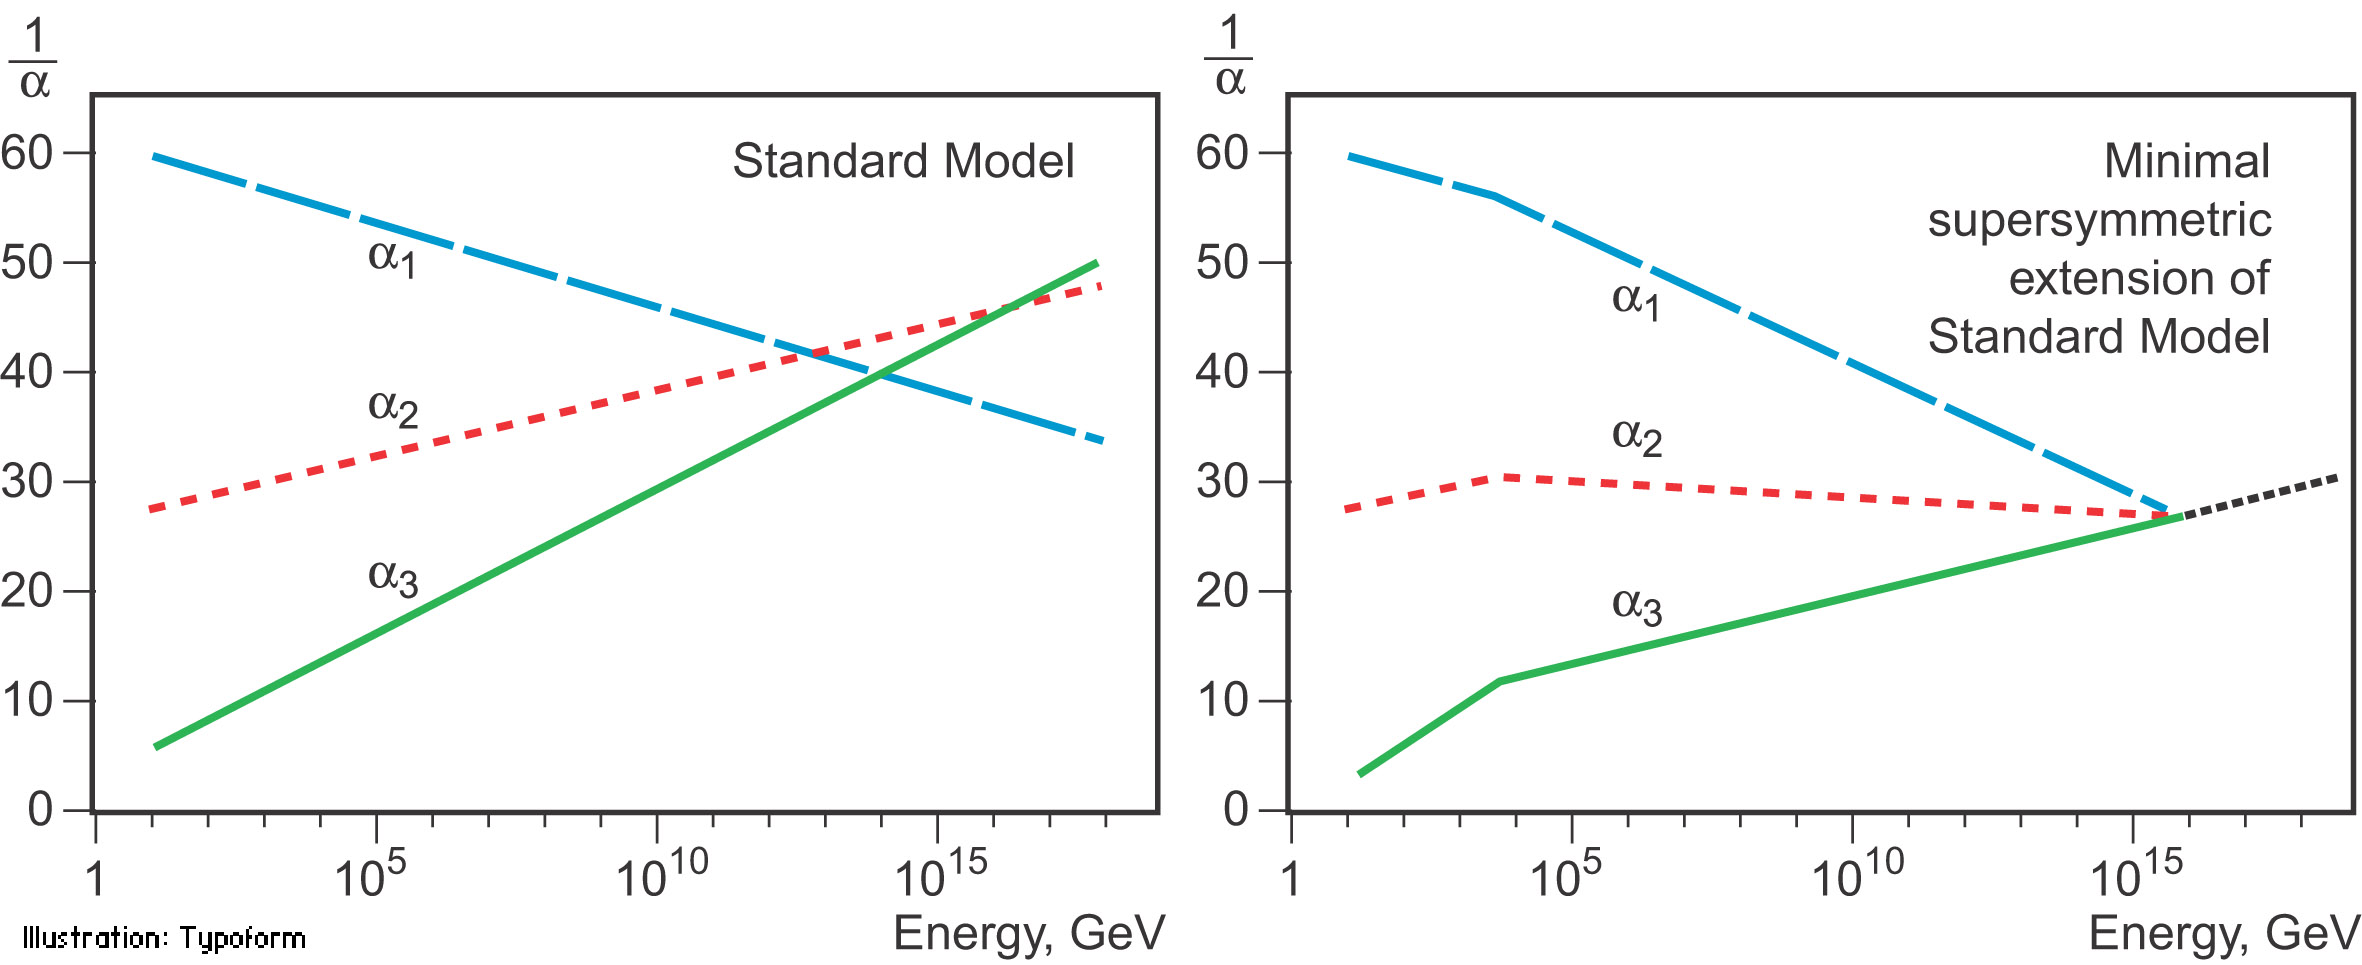
\includegraphics[width=\textwidth]{theory/alphaRunning}
			\caption{\label{fig:alphaRunning} The inverse couplings of electromagnetic (dashed blue), weak (dashed red) and strong (solid green) interactions with the \ac{SM} (left) and a supersymmetric model (right). In the \ac{SM} the three lines do not meet at one point, but with the introduction of supersymmetry, and assuming that the supersymmetric particles are not heavier than about 1 \TeV, they do meet.}
		\end{figure}		

		\ac{SUSY} introduces a space-time symmetry that relates bosons to fermions and vice-versa, via a transformation of the form of:  

		\begin{equation}
		\label{eq:susy_transformation}
			Q \ket{\mathrm{fermion}} = \ket{\mathrm{boson}}, \qquad Q \ket{\mathrm{boson}} = \ket{\mathrm{fermion}}
		\end{equation}

		\noindent For each \ac{SM} particle there exists a supersymmetric partner, generally called \textit{sparticle} (where the s stands for “scalar”), with a spin difference of $\Delta s = 1/2$. Each pair of partners is arranged in a so-called \textit{supermultiplet}. The two components have same masses and quantum numbers, but different spin, due to their relation to the $Q$ operator (and its properties). 

		\textit{Sleptons} and \textit{squarks} interact as their \ac{SM} equivalent. The superpartners of the left-handed fermion components couple weakly, while the superpartners of the right-handed \ac{SM} fermion components do not couple at all. 
		Gauge supermultiplets contain a vector boson and two spin-$\frac{1}{2}$ fermions. Spin-1 bosons are arranged in gauge multiplets, and their superpartners, referred to as \textit{gauginos}, are spin-$\frac{1}{2}$ fermions. Unlike the \ac{SM}, the Spin-0 Higgs boson has two supermultiplets containing sparticles with different weak isospin values, referred to as $H_u$ and $H_d$, which are required to give mass to both the up- and down-type sparticles. Higgs \ac{SUSY} partners are called the \textit{Higgsinos}.

		As of today, \ac{SUSY} particles have not been observed, resulting in the assumption that \ac{SUSY} must be a broken symmetry, otherwise superpartners would have the same masses as their \ac{SM} equivalent. However, if sparticles were to be too heavy (close to the Planck scale), the hierarchy problem would be re-introduced and therefore would still remain unsolved. The \emph{soft} \ac{SUSY} breaking mechanism, described in Section~\ref{sec:MSSM}, overcomes this problem by imposing constraints on the masses of sparticles to a range that can be experimentally explored. 		


		\subsection{Minimal Supersymmetric Standard Model}
		\label{sec:MSSM}
			
			There does not exist a unique extension of a supersymmetric \ac{SM}, \ie\ \ac{SUSY} is not a well-defined model but it is more a framework within which various \ac{SM} extensions can be derived.
			The \ac{MSSM} is a minimal supersymmetric extension of the \ac{SM}, defined by essentially doubling up the number of particles in the \ac{SM} theory in order to include all the \ac{SM} particles as well as their corresponding superpartners.

			\subsubsection*{Soft SUSY breaking}
				
				The mass spectrum of the \ac{SUSY} particles must sit somewhere at a larger scale than the \ac{SM} one, as supersymmetric particles have not been discovered at the mass scale of their \ac{SM} partners. This gives us a hint that supersymmetry cannot be an exact symmetry and therefore it is broken. There has to be an analogy here with the electroweak symmetry breaking discussed in~\ref{sec:ewksb}, where the symmetry is broken by a non-zero \ac{VEV}. The mechanism must be spontaneous in order for the broken supersymmetry to still provide a solution to the hierarchy problem: a big alteration of the relationship between the fermionic and scalar couplings will result in a non-cancellation of the corrections to the Higgs mass squared parameter.
				% from SM fermions by their SUSY partners correction terms. 	
				This equates to adding terms to the \ac{SUSY} Lagrangian which are gauge invariant and violate \ac{SUSY}, but contain only masses and couplings with positive mass dimension. The total Lagrangian is defined as;

				\begin{equation}
				\label{eq:soft_sb}
					\mathcal L_{\mathrm{MSSM}} = \mathcal {L_{\mathrm{SUSY}}} + \mathcal {L_{\mathrm{soft}}}
				\end{equation}

				\noindent where all the additional terms are contained within $\mathcal {L_{\mathrm{soft}}}$ and the original \ac{SUSY} invariant interaction terms are contained within $\mathcal {L_{\mathrm{SUSY}}}$. A new set of parameters is then introduced into this \ac{SM} extension. These parameters determine the mixing between the flavour eigenstates and the \ac{SUSY} phenomenology, which will be discussed in Section~\ref{sec:SUSYPheno}. 

				% Although the actual mechanism that breaks \ac{SUSY} is unknown, there are several proposed ideas that have been studied in depth, but this will not be discussed any further. The general approach involves a coupling to a separate hidden sector of fields, in which, spontaneous \ac{SUSY} breaking occurs [25]. The hidden sector then communicates the \ac{SUSY} breaking to the MSSM sector via messenger fields such that the soft \ac{SUSY}-breaking terms are generated. 

				% A large amount of theoretical effort has been spent trying to understand the mechanism for soft \ac{SUSY} breaking in order to produce the desired superpartner masses and interaction properties. Among these three most studied mechanisms are; 

				% \begin{itemize}
				% 	\item gravity-mediated supersymmetry breaking, also known as mSUGRA (minimal supergravity), which communicates supersymmetry breaking to the supersymmetric \ac{SM} through gravitational interactions~\cite{PhysRevLett.49.970}; 
				% 	\item gauge-mediated supersymmetry breaking (GMSB) which communicates supersymmetry breaking to the supersymmetric \ac{SM} through the \ac{SM}'s gauge interactions~\cite{ARBEY2012162}; 
				% 	\item anomaly-mediated supersymmetry breaking (AMSB), a special type of gravity-mediated supersymmetry breaking, that communicates supersymmetry breaking to the supersymmetric \ac{SM} through the conformal anomaly~\cite{Randall:1998uk, Giudice:1998xp}
				% \end{itemize}



			\subsubsection*{MSSM mass spectrum}

				As per the \ac{SM} gauge bosons, the gaugino masses are affected by electroweak symmetry breaking. The new states, introduced in the $\mathcal L_{\mathrm{soft}}$, mix to form the mass eigenstates of the sparticles. The neutral Winos ($\tilde{W}^0$), Binos ($\tilde{B}^0$), and Higgsinos ($\tilde{H}^0$) mix to form the four \textit{neutralinos} $\tilde{\chi}^0_i$ ($i=1,2,3,4$):

				\begin{equation}
				\label{eq:neutralino_mixing}
					\begin{pmatrix}  \ninoone \\ \ninotwo \\ \ninothree \\ \ninofour \end{pmatrix}	
					= 
					\begin{pmatrix}
						M_1 & 0 & - c_\beta s_W m_Z &  c_W s_\beta m_Z  \\
						0 & M_2 & c_\beta c_W m_Z  &  - c_W s_\beta m_Z \\
						- c_\beta s_W m_Z  & c_\beta s_W m_Z  & 0 & - \mu \\ 
						s_\beta c_W m_Z  & - s_\beta c_W m_Z & - \mu & 0  
					\end{pmatrix}
					\begin{pmatrix}
						\tilde{B}^{0} \\
						\tilde{W}^{0} \\
						\tilde{H}^{0}_u \\
						\tilde{H}^{0}_d
					\end{pmatrix}
				\end{equation}

				\noindent Here, $c_{\beta} = \cos \beta$,  $(s_{\beta}) = \sin \beta$, $c_W = \cos \theta_W$ and $(s_W) = \sin \theta_W$. $M_1$, $M_2$ are related to gaugino masses and $\mu$ to Higgsinos mass, $\tan \beta$ is the ratio of the \ac{VEV}s of the two Higgs doublet fields, $\theta_W$ is the ratio of the electroweak coupling constants and, $m_Z$ ($m_W$) is the mass of the \Zboson\ (\Wboson) boson. The neutralino indices are conventionally assumed to increase with their masses. The charged winos ($\tilde{W}^{\pm}$) and Higgsinos ($\tilde{H}^{\pm}$) mix to form four \textit{charginos}, $\tilde{\chi}^{\pm}_i$ ($i=1,2$):

				\begin{equation}
				\label{eq:chargino_mixing}
						\begin{pmatrix}  \tilde{\chi}^{\pm}_1 \\ \tilde{\chi}^{\pm}_2 \end{pmatrix}	
						= 
						\begin{pmatrix}
							M_2 & \sqrt{2} m_W s_\beta \\
							\sqrt{2} m_W c_\beta & \mu  
						\end{pmatrix}
						\begin{pmatrix}
							\tilde{W}^{\pm} \\
							\tilde{H}^{\pm}
						\end{pmatrix}
				\end{equation}

				Charginos and neutralinos mix as described in Equation~\ref{eq:chargino_mixing} and~\ref{eq:neutralino_mixing} and will be referred to as bino-like, wino-like or higgsino-like depending on their phenomenology. Gluinos do not mix as they carry colour charge. 

				The Higgs sector is also affected. There are five mass eigenstates, $h^0$, $H^0$, $A^0$, and $H^{\pm}$. These, together with the other \ac{MSSM} particles are listed in Table~\ref{tab:MSSM_particles}. 
				
				\begin{table}[!htb]\centering\caption{\ac{SUSY} particles in the \ac{MSSM}}
				\renewcommand{\arraystretch}{1.4}
					\begin{tabular}{lclc}
						\toprule
						\textbf{Name} & \textbf{Spin} & \textbf{Gauge Eigenstates} & \textbf{Mass Eigenstates} \\
						\toprule
						
						\multirow{3}{*}{Squarks ($\tilde{q}$)} & \multirow{3}{*}{0} 
						& $\tilde{u}_L$ $\tilde{u}_R$ $\tilde{d}_L$ $\tilde{d}_R$ & (same) \\
						& & $\tilde{c}_L$ $\tilde{c}_R$ $\tilde{s}_L$ $\tilde{s}_R$ & (same) \\
						& & $\tilde{t}_L$ $\tilde{t}_R$ $\tilde{b}_L$ $\tilde{b}_R$ & $\tilde{t}_1$ $\tilde{t}_2$ $\tilde{b}_1$ $\tilde{b}_2$ \\ 
						\midrule

						\multirow{3}{*}{Sleptons ($\tilde{l}$)} & \multirow{3}{*}{0} 
						& $\tilde{e}_L$ $\tilde{e}_R$ $\tilde{\nu}_L$ & (same) \\
						& & $\tilde{\mu}_L$ $\tilde{\mu}_R$ $\tilde{\nu}_L$ & (same) \\ 
						& & $\tilde{\tau}_L$ $\tilde{\tau}_R$ $\tilde{\nu}_{\tau}$ & $\tilde{\tau}_1$ $\tilde{\tau}_2$ $\tilde{\nu}_{\tau}$ \\ 
						\midrule
						
						Higgs bosons & 0 & $H_u^0$ $H_d^0$ $H_u^+$ $H_d^-$ & $h^0$ $H^0$ $A^0$ $H^{\pm}$ \\ 
						\midrule 

						Neutralinos ($\tilde{\chi}_j^0$)   & 1/2 & $\tilde{B}^0$ $\tilde{W}^0$ $\tilde{H}_u^0$ $\tilde{H}_d^0$ & $\tilde{\chi}_1^0$ $\tilde{\chi}_2^0$ $\tilde{\chi}_3^0$ $\tilde{\chi}_4^0$\\
						Charginos ($\tilde{\chi}_i^{\pm}$) & 1/2 & $\tilde{W}^{\pm}$ $\tilde{H}_u^+$ $\tilde{H}_u^-$ & $\tilde{\chi}_1^{\pm}$ $\tilde{\chi}_2^{\pm}$ \\
						\midrule

						Gluino & 1/2 & $\tilde{g}$ & (same) \\
						Gravitino & 3/2 & $\tilde{G}$ & (same) \\ 					
						\bottomrule
					\end{tabular}						
				\label{tab:MSSM_particles} 
				\end{table}


				In the \ac{MSSM} the squark sector is specified by the mass matrix in the basis $(\tilde{q}_L, \tilde{q}_R)$ with $\tilde{q} = \tilde{t}$ or $\tilde{b}$~\cite{Haber:1984rc}. A rotation matrix can be defined also for left- and right-handed squarks and sleptons, although in the \ac{MSSM} the mixing is assumed to be non-zero only for the third-generation scalar partners. Stop (\stopL, \stopR), sbottom (\sbottomL, \sbottomR), and stau (\stauL, \stauR) rotate into mass eigenstates, \stopone, \stoptwo, \sbottomone, \sbottomtwo, \stauone, \stautwo, respectively, as described in Equation~\ref{eq:3rdgen_mixing}~\cite{Hidaka:2000cm}: %As with the neutralinos and charginos, the lower the index, the lighter the particle is. 

				\begin{equation}
				\label{eq:3rdgen_mixing}
					\mathcal {M}_{\tilde{q}}^2 = 
					\begin{pmatrix}
						m_{\tilde{q}_L}^2 & a_q m_q \\
						a_q m_q & m_{\tilde{q}_R}^2
					\end{pmatrix}
				\end{equation}

				\noindent with 

				\begin{align}
				\label{eq:msqL}
					\begin{split}
						m_{\tilde{q}_L}^2 & = M_{\tilde{Q}}^2 + m_Z^2 \cos 2\beta \left ( I_3^{q_L} - e_q \sin^2 \theta_W \right ) + m_q^2 ,
						\\ 
						m_{\tilde{q}_R}^2 & = M_{{\{ \tilde{U},\tilde{D} \}}}^2 + m_Z^2 \cos 2\beta\, e_q \sin^2 \theta_W  + m_q^2 , 
						\\
						a_q m_q & = 
						\begin{cases}
							\left ( A_t - \mu \cot \beta \right ) m_t\, , \, (\tilde{q} = \tilde{t}) \\  
							\left ( A_b - \mu \tan \beta \right ) m_t\, , \, (\tilde{q} = \tilde{b})  
						\end{cases}
					\end{split}
				\end{align}

				\noindent Here, $I_3^{q_L}$ is the third component of the weak isospin and $e_q$ the electric charge of the quark $q$. $M_{{\{ \tilde{Q},\tilde{U},\tilde{D} \}}}$ and $A_{t,b}$ are soft \ac{SUSY}–breaking parameters, $\mu$ is the higgsino mass parameter, and $\tan \beta$, as previously mentioned, is the ratio of Higgs field \ac{VEV}s. By diagonalising the matrix in Equation~\ref{eq:3rdgen_mixing} one gets the mass eigenstates 
				
				\begin{align}
					\tilde{q}_1 & = \tilde{q}_L \cos \theta_{\tilde{q}} + \tilde{q}_R \sin \theta_{\tilde{q}} \\
					\tilde{q}_2 & = - \tilde{q}_L \sin \theta_{\tilde{q}} + \tilde{q}_R \cos \theta_{\tilde{q}}
				\end{align}
				
				\noindent with the mass eigenvalues $m_{\tilde{q}_1}$, $m_{\tilde{q}_2}$ ($m_{\tilde{q}_1} < m_{\tilde{q}_2}$ ) and the mixing angle $\theta_{\tilde{q}} \left (- \pi / 2 < \theta_{\tilde{q}} \leq \pi / 2 \right )$. 
				


		\subsection{Phenomenology of Supersymmetry}
		\label{sec:SUSYPheno}

			As previously mentioned, the introduction of \ac{SUSY} particles overcomes the problem of an unnatural fine-tuning to the Higgs mass due to its quadratic corrections.%, given that the stops have masses typically around 1 TeV.

			\subsubsection*{$R$-parity}
				
				The most general \ac{MSSM} can contain operators that violate baryon and/or lepton number, thus allowing the decay of the proton. The non-observation of proton decays forbids the existence of such terms. A possibility to avoid these operators is to introduce a new discrete symmetry named $R$-parity. The conserved quantum number is defined as;

				\begin{equation}
					P_R = \left ( -1 \right )^{3 \left (B - L \right )+ 2s}
				\end{equation}

				\noindent where $B$, $L$, and $s$ are the baryon, lepton, and spin number, respectively.	

				The \ac{SM} particles have $R = 1$ and \ac{SUSY} partners have $R=-1$. When $R$-parity conservation is imposed on \ac{MSSM} models, the mixing between particles and sparticles cannot occur, resulting in the number of \ac{SUSY} particles to be even at every interaction vertex. Furthermore, all sparticles must be pair-produced and the \ac{LSP} has to be stable and can be a good Dark Matter candidate. %Heavier sparticles can only decay to odd numbers of it.

				Although \ac{SUSY} searches in an $R$-parity violating (RPV) scenario have been extensively investigated by the particle-physics community, in this work only $R$-parity conserving (RPC) models, where the \ninoone\ is assumed to be the \ac{LSP}, were considered.

			\subsubsection*{Phenomenological \ac{MSSM} (pMSSM)}

				As mentioned in~\ref{sec:MSSM}, once the \ac{SUSY} soft breaking occurred, the unconstrained \ac{MSSM} has more than 100 parameters in addition to the \ac{SM} ones. This makes the \ac{SUSY} searches, \eg\ finding regions in parameter space that are consistent with the data, rather impractical. However, the number of free parameters can be reduced down to 19 if the following  assumptions are made; 

				\begin{itemize}
					\item there is no new source of CP-violation (CKM matrix is the only source)
					\item there are no \ac{FCNC}
					\item the masses of the first- and second-generation sfermions are identical (first- and second-generation universality)
				\end{itemize}
				
				\noindent The introduction of such constraints allows the definition of the the so-called \ac{pMSSM}, summarised in Table~\ref{tab:MSSM_mainFreePar}.
				
				\begin{table}[!htb]\centering\caption{Parameters in the pMSSM.}
				\renewcommand{\arraystretch}{1.3}
					\begin{tabular}{llc}
					\toprule
					\textbf{Parameter} & \textbf{Description} & \textbf{N. of parameters} \\ 
					\toprule

					$M_1$, $M_2$, $M_3$ & Bino, Wino and gluino masses & 3 \\ \midrule

					$M_{A}$	& pseudo-scalar Higgs boson mass	& 1 \\\midrule
					$\mu$  & higgsino mass & 1 \\\midrule

					$m_{\tilde{q}}$, $m_{\tilde{u}_R}$, $m_{\tilde{d}_R}$, & first- and second-generation squark masses & 3 \\
					$m_{\tilde{Q}_L}$, $m_{\stop}$, $m_{\sbottom}$ & third generation squark masses	&  3 \\\midrule

					$m_{\tilde{l}}$, $m_{\tilde{e}_R}$ & first- and second-generation slepton masses	 & 2 \\
					$m_{\tilde{L}}$, $m_{\stauR}$ & third-generation slepton masses	& 2 \\\midrule

					$A_t$, $A_b$, $A_{\tau}$ & third-generation trilinear couplings	& 3 \\\midrule

					$\tan \beta$ & two-higgs-doublet fields \ac{VEV}s ratio & 1 \\ 
					\bottomrule
					\end{tabular}
				\label{tab:MSSM_mainFreePar} 
				\end{table}

				\noindent Such parameter space is still rather large and it makes \ac{pMSSM} searches extremely challenging and difficult to exclude. To overcome this problem \textit{simplified models} are introduced. In other words, a certain signal process is extracted from the model and only particles contributing to a certain decay mode will be considered, \eg\ $\stopone \ra t + \ninoone$ only targets the 2-body decay ignoring the remaining \ac{SUSY} mass spectrum. The number of parameters will then reduce to 2; \mstop\ and \mLSP, allowing the reinterpretation of the results and providing a powerful tool to constrain various models. 

				In this work only analyses based on such simplified models will be presented. 

			\subsubsection*{Phenomenology of the top squark}

				Figure~\ref{fig:susy_13TeV_xsec} shows \ac{SUSY} particles production cross-sections in \pp\ collisions at $\sqrt{s} = 13 \TeV$ for squarks that do not contribute to gluino production diagrams and vice versa, \ie\ treating squarks and gluinos as \textit{decoupled} by making the cross-section of squark pair-production the same for all families. While gluino pair-production cross-sections are fairly large, \ac{SUSY} electroweak production cross-sections of neutralinos and charginos are considerably lower. Slepton production cross-section, which is not displayed, would sit just below higgsino-like chargino/neutralino production cross-section. 

				\begin{figure}[!htb]
					\centering
					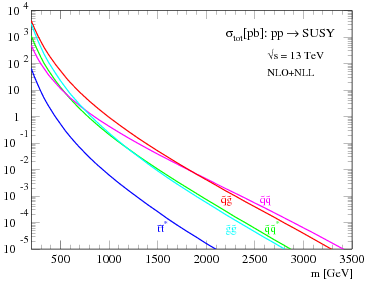
\includegraphics[width=\textwidth]{theory/SusyXSec13TeV}
					\caption{\label{fig:susy_13TeV_xsec} NLO+NLL production cross-sections as a function of mass at $\sqrt{s} = 13 \TeV$~\cite{Borschensky:2014cia}}
				\end{figure}

				There exists various decay modes of pair-produced stops, depending on the masses of the decay products; 

				\begin{itemize}
					\item $\stop \ra t\ \ninoone$
					\item $\stop \ra b\ \chinoonepm \ra b\  W\  \ninoone$ (on/off-shell \Wboson) or $\stop \ra b\  W\  \ninoone$ (off-shell top)
					\item $\stop \ra c\ \ninoone$
					\item $\stop \ra b\ f\ f'\ \ninoone$
				\end{itemize} 

				Figure~\ref{fig:stop_topologies} shows a schematic representation of the parameter space ($m_{\stopone}, m_{\ninoone})$ and the different regions where each of the above-mentioned process dominates. %In particular, $\stop \ra b\ \chinopm$ is allowed when $m_{\nino} < m_{\chinopm} < \mstop - m_b$.

				\begin{figure}[!htb]
					\centering
					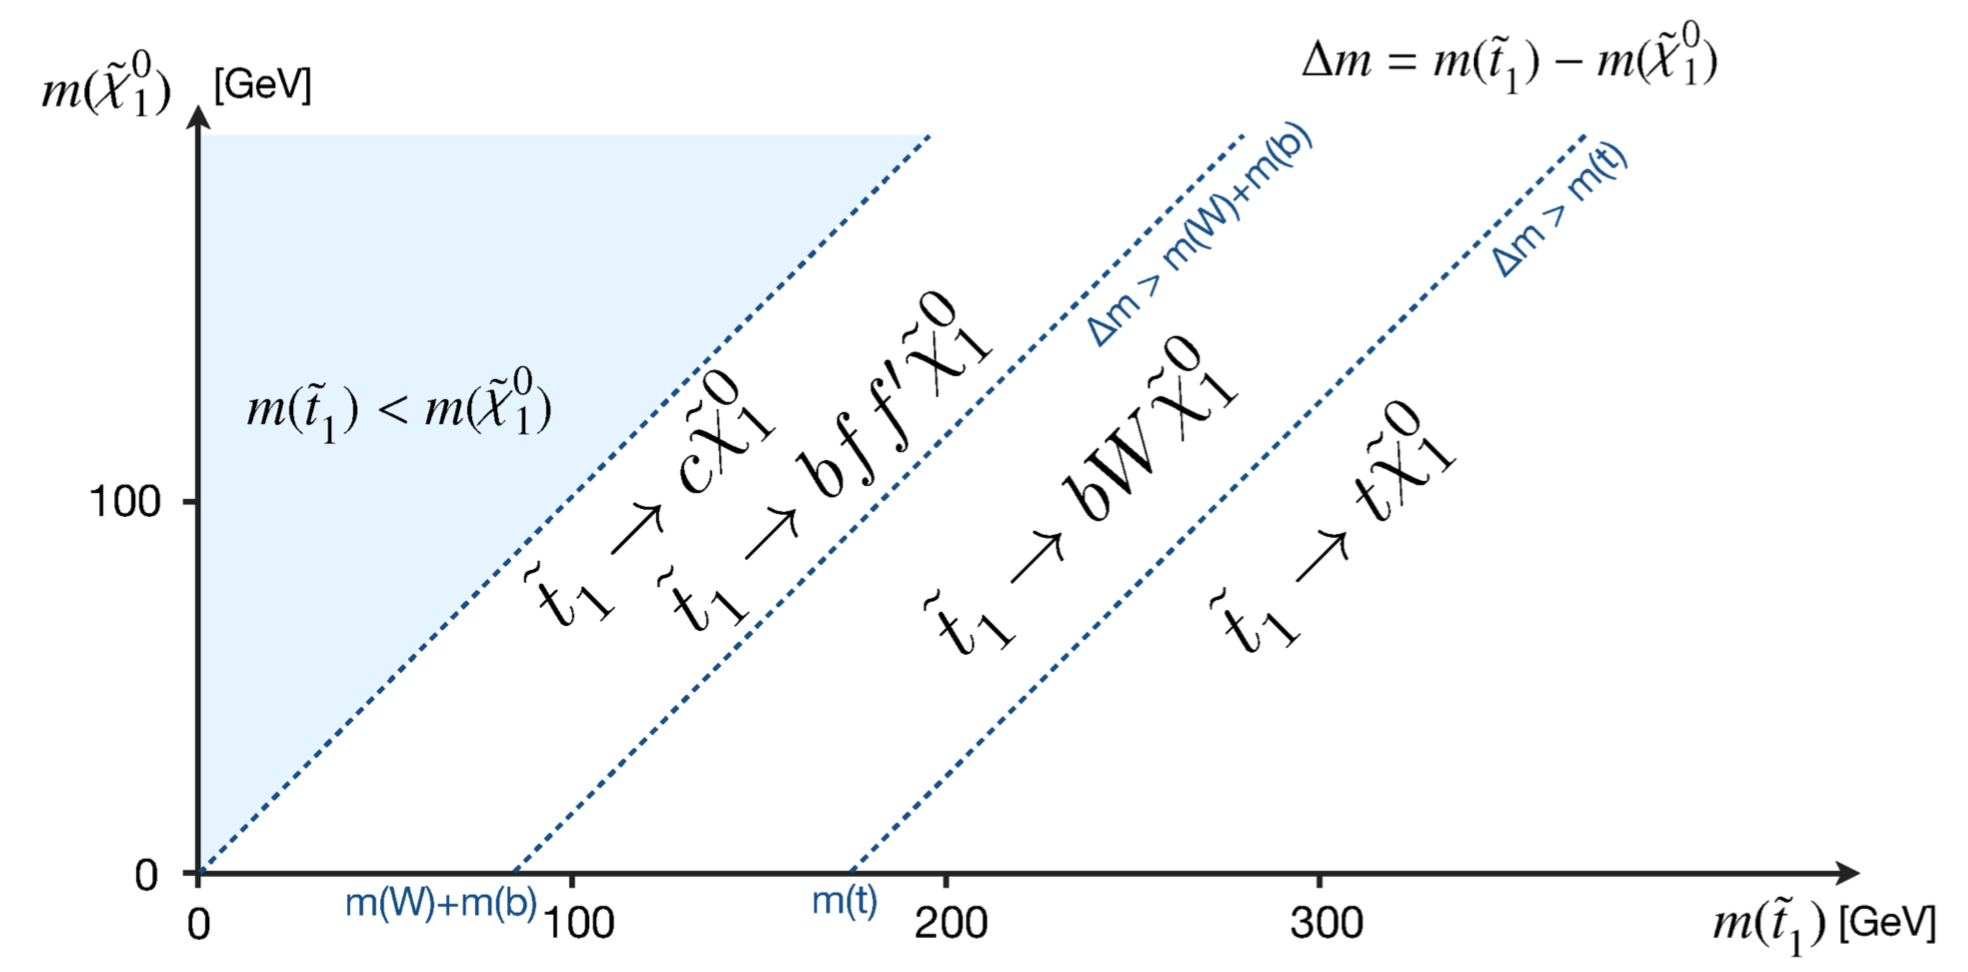
\includegraphics[width=\textwidth]{theory/3rd_gen_searches.png}
					\caption{\label{fig:stop_topologies} Illustration of stop decay modes in the ($m_{\stopone}, m_{\ninoone})$ mass place where the \ninoone\ is assumed to be the \ac{LSP}. The dashed blue lines indicate thresholds separating regions where different processes dominate.}
				\end{figure}

				In the models considered in this work, either \ninotwo\ or \chinoonepm\ is assumed to be the so-called \ac{NLSP}. Three different decay scenarios were considered: (a) where both top squarks decay via $\stop\rightarrow t^{(*)}\ \ninoone$\footnote{The symbol (*) indicates the off-shell production}; (b) at least one of the stops decays via $\stop\rightarrow b\ \chinoonepm \rightarrow b\ \Wboson^{(*)}\ \ninoone$; (c) where $m_{\ninotwo}$ is small enough to allow one stop to decay via $\stop\to t\ \ninotwo \to h/Z\ \ninoone$. Here, $h$ is the \ac{SM} Higgs boson (125 GeV), as illustrated in Figure~\ref{fig:feynDiagModels}(a)$-$(c), respectively. Furthermore, top squarks can also be indirectly produced through the so-called gluino-mediated stop production, as shown in Figure~\ref{fig:feynDiagModels}(d).

				\begin{figure}[!htb]
					\begin{center}
						\subbottom[$\stop\ra t^{(*)}\ninoone$]{
							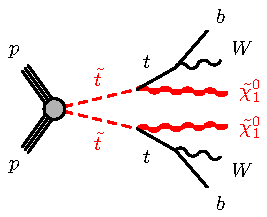
\includegraphics[width=0.25\textwidth]{theory/stst-bqqbqqN1N1-tt}}\hspace{0.05\textwidth}
						\subbottom[$\stop\ra b\ \chinoonepm\ra b \Wboson^{(*)}\ninoone$]{
							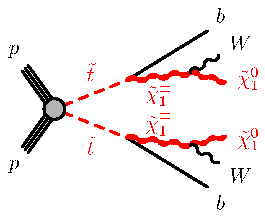
\includegraphics[width=0.25\textwidth]{theory/stst-bbWWN1N1}}\hspace{0.05\textwidth}
						\subbottom[$\stop\ra t\ \ninotwo\to h/Z\ \ninoone$]{
							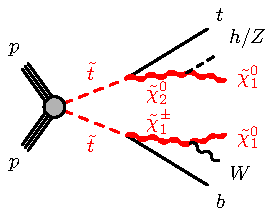
\includegraphics[width=0.25\textwidth]{theory/stst-tbhWN1N1}}\hspace{0.05\textwidth}
						\subbottom[$\gluino \ra t\ \stop\ra t\ \ninoone +$soft]{
							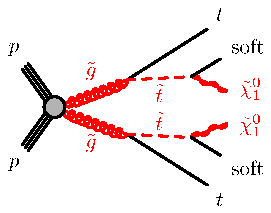
\includegraphics[width=0.25\textwidth]{theory/gogo-tsofttsoftN1N1-stst}}\hspace{0.05\textwidth}
					\end{center}
					\caption{Diagrams of the decay topologies of the signal models considered in this work. The term ``soft" refers to decay products that have transverse momenta below the detector thresholds.}
					\label{fig:feynDiagModels}
				\end{figure}

				Third-generation \ac{SUSY} analyses, \eg\ stop pair-production ($\stop\stop$) or sbottom pair-production ($\sbottom\sbottom$) are very challenging, due to the cross-section being around a factor of six smaller than \ttbar\ production (when $m_{\stopone} \sim m_t$), which usually is one of the main backgrounds. Furthermore, the cross-section of such processes dramatically decreases with increasing $m_{\tilde{q}}$. Nonetheless, for example, searches for direct \stopone\ production with $\stopone \ra t + \ninoone$ are sensitive in a scenario where $m_{\stopone} \gg m_t + m_{\ninoone}$ as the large \met, from the neutralinos, provides discriminating power for \ttbar\ rejection. Further details will be discussed in Chapter~\ref{ch:stop_ana}.
				